\documentclass[conference]{IEEEtran}
\usepackage{cite}
\usepackage{array}
\usepackage{graphicx}
\usepackage{amsthm}
\usepackage{amsmath}
\usepackage{listings}	% Used to add code
\lstset{language=Java}


\usepackage{float} %used to force figures in a position
\hyphenation{op-tical net-works semi-conduc-tor}

\theoremstyle{definition}
\newtheorem{definition}{Definition}[section]

\begin{document}
\title{Building a Compilator on Java for a mini-C Programming Language}

\author{\IEEEauthorblockN{J. Agust\'{i}n Barrachina}
\IEEEauthorblockA{IEEE Student Member\\
\'{E}cole Polytechnique\\
Universit\'{e} Saclay-Paris}
\and
\IEEEauthorblockN{Phil\'{e}mon Poux}
\IEEEauthorblockA{\'{E}cole Polytechnique\\
	Universit\'{e} Saclay-Paris}}
\maketitle

\tableofcontents
\newpage

\begin{abstract}
In this project, a compilator was created to generate a x86-64 assembler code from a C fragment called mini-C.
This is a 100\% C-compatible fragment, in the sense that any Mini C program is also a C program.
\end{abstract}

\IEEEpeerreviewmaketitle

\section{Introduction}
\textit{"Optimizing compilers are so difficult to get right that we dare say that no optimizing compiler is error-free! Thus, the most important objective in writing a compiler is that it is correct"}\cite{DRAGON_BOOK}

The reader is suppose to have some basic knowledge of C and for that reason almost no explanation regarding that language will be treated in this report. For further information about C language refer to \cite{LANGUAGE_C}.

Simply stated, a Compiler is a program that can read a code written in a specific programming language and translate it into an equivalent code of another language. A fairly good analogy can be made by a translator between two different languages like Spanish and French for example.

The objective of this project is to create a compiler for a fragment of C denominated \textit{Mini C} towrds a reasonably effective code x86-64. In this project, a ".s" file will be created containing the translation between the C file to assembly. After the file is generated, the use of another compiler will be needed to produce the final output file that can be run by the computer.

General knowledge of x86-64 assembly and the functioning of processors will also be required. The concept of the stack and registers like the callee saved and the caller saved must be clear for the reader.

\subsection{Mini C}
\subsubsection{What it does}
\textit{Mini C} is a fragment of the language C which contains integers and pointers to structures. \textit{Mini C} is 100\% compatible with C in the sense that every \textit{Mini C} program is also a C program. This will enable to use a C compiler such us \textbf{gcc} to use as reference.

\textit{Mini C} can deal both with integers and structures. It can even support pointers inside structures to other structures or to the same structure in order to create lists for example. Mini is a Turing Complete language thus, despite its small structure, every single code in C can be reduced to \textit{Mini C}.

\subsubsection{What it doesn't}
%TODO: ADD STUFF NOT IMPLEMENTED.
\textit{Mini C} can deal both with integers and structures. But it doesn't work with any other types of variables such as floating point numbers or characters directly.

%The function \textit{sizeof} is not yet implemented. The compiler will %read it correctly and will know the program is correctly written but it %will not know how to translate \textit{sizeof} resulting in an %incomplete and broken assembly code.

\textit{Mini C} doesn't implement a for loop. Even though is almost the same as implementing a while loop. It was not believed to be relevant the implementation of it as an academic objective as the implementation of it will only require time but will not help in the better understanding of a compiler.
 
The "++" and "- -" commands to increase or decrease a variables value were not implemented as well.

\subsubsection{Known bugs and work to be done}
%TODO: add bugs

There was no real communication between the typer and the RTL (section \ref{sec:RTL}) generation code. For which reason, the toRLT function had to create in some cases some information already treated. This was not only working twice but also made the syntax class longer and more difficult to read. It is work for the future to create a better communication between both parts.

In the program, global structures were not yet implemented, although the code is prepared for it. In the section of code which it should be done, a throw error is prompt saying that the global structures are not yet implemented. Other uses with structures are implemented but prone to bugs as no enough debugging was made in this area. 

Although the compiler computes "$5 + 4$" directly as $9$, it will fail to do so when more complex integer operations are done like "$4 * 9 + (4 \&\& 0)$". It is to be done more optimization on this side. Jumps are also always done by the program itself and the compiler will not compute a "if(1)" as a direct jump to the section of code inside the if loop.

The Appel \& George algorithm can be applied for coloring the interference graph (section \ref{sec:coloring}) in order to achieve better registers assignments for a better optimized assembly code.

\subsection{Structure of a Compiler}\label{sub_structure_of_a_compiler}

A compiler can be divided into two parts. The \textit{analysis} (front end) and the \textit{synthesis} (back end)

The \textit{analysis} brakes the source program into constituent pieces and imposes a grammatical structure of them in order to create a intermediate representation of the source program. During this part, syntactical formation and semantical unsound is checked. The analysis also collects information about the source program and stores it in a data structure called a \textit{symbol table} which will be used by the \textit{synthesis} part.

The \textit{synthesis} part makes use of the \textit{symbol table} and the intermediate representation constructed by the analysis part and creates the target program.

A more detailed diagram of the structure can be seen in figure \ref{fig_struct_of_compilator}. Where the last part (Code Generation) correspond to the \textit{synthesis} phase and the rest are all from the \textit{analysis} phase. The diagram is longer that the one displayed, having also a converser from the assembler to the machine language and from there to the executable code. But in this project, those stages are not treated.

\begin{figure}[H]
\centering
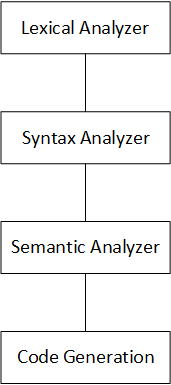
\includegraphics[width=3cm]{images/Diagram.png}
\caption{Structure of a Compiler}
\label{fig_struct_of_compilator}
\end{figure}

\section{Lexical Analyzer} \label{sec:lexical-Analizer}
A lexical analyzer (\textit{Lexer}) is the first front-end step in compilers, matching keywords, comments, operators, etc, and generating a token stream for parsers called \textit{lexemes} consisting of a \textit{token name} and the \textit{attribute value}.
The \textit{token name} is an abstract symbol that will be used during syntax analysis, while the \textit{attribute value} is an entry in the \textit{symbol table} (discussed on \ref{sub_structure_of_a_compiler}) which will be used during the semantic analysis and the code generation.

The Lexer reads input from the programming language to compile (mini c in our case) and matches it against regular expressions and runs a corresponding action if such an expression is matched.

To make the Lexer are going to use:
\begin{itemize}
	\item Regular Expressions: To describe the lexemes
	\item Finite Automata: To recognize the expressions
\end{itemize}
\subsection{Regular Expressions}
The concept of regular expression arose in the 1950's when the American mathematician Stephen Cole Kleene formalized the description of a regular language.

A regular expression is a sequence of characters that define a search pattern. In other words, there are a conjunction of letters and digits that follow a certain rule.

Let us define \textit{letter} as any letter in the Latin alphabet and \textit{digit} any number [0-9]. Then we can define rules as follow:
\begin{equation}
0 | [1-9] (<digit>* | [])\label{reg_expr_example}
\end{equation}

Last equation \ref{reg_expr_example} is a declaration of a decimal digit. The "$|$" is a logic or, it means, either the digit is 0 or it will be another thing. If it is not only 0, the number cannot start by 0 in C syntax, so it must start with a digit different from 0, which is range from 1 to 9 (encoded as [0-9]). Secondly, this digit can be followed by either nothing (represented by: []) or by any digit for as many digits are they must be. The format $<$rule$>$* means the repetition of a rule for as many times as necessary, or no repetition at all.

% We could add another example here, for example a comment line or sth.
\subsection{Finite Automata}
A \textit{finite automata} is basically a binary graph which just say "yes" or "no" by means of a \textit{recognizer} to each possible string.

There are two different classes of automatas:
\begin{enumerate}
	\item \textit{Nondeterministic Finite Automata} (NFA)
	\item \textit{Deterministic Finite Automata} (DFA)
\end{enumerate}
The first class (NFA) have no restrictions on the labels of their edges. A symbol can label several edges out of the same state. The DFA on the other hand have for each state and symbol exactly one edge with that symbol leaving that state.
%translate to english...

\subsection{Implementation}

For the lexical analyzer, a flex library was used \cite{JFLEX}. A .flex file was created and then, by means of jflex, converted to the final java class.

Jflex lexers are based on a DFA automata. For more information about jflex library please refer to \cite{JFLEX_MANUAL}.

The work of the lexer was only to read input from the file and create new symbols (\textit{lexemes}) containing the information as explained in \ref{sec:lexical-Analizer}.

\section{Syntax Analyzer} \label{sub_syntax_analyzer}

The syntax of a programming language describes the proper form of its programs.

The \textit{syntax analyzer} or \textit{parser} uses the first component of the \textit{lexemes}, the \textit{tokens}. The \textit{parser} creates some kind of tree representation that depicts the grammatical structure of the token stream called the \textit{syntax tree}. In this tree, each node represent an operation and the children of the node represent the arguments of that operation.

\begin{figure}[H]
	\centering
	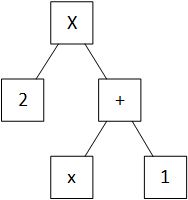
\includegraphics[width=3cm]{images/syntax_tree.png}
	\caption{Syntax Tree Example}
	\label{fig_syntax_tree_example}
\end{figure}

On figure \ref{fig_syntax_tree_example} an example of a tree representation can be seen. Many syntaxes can be the cause of that tree, for example, both \ref{(2*((x)+1))} and \ref{2*(x+1)} can be used to generate such tree.

\begin{equation}
2*(x+1)
\label{2*(x+1)}
\end{equation}

\begin{equation}
(2*((x)+1))
\label{(2*((x)+1))}
\end{equation}

\subsection{Implementation}

The Syntax Analyzer was done using CUP, a parser generator for java \cite{CUP}.

In that file, precedence where applied to each operator using the following table:
\begin{table}[H]
	\begin{center}
	\begin{tabular}{||c c||}
		\hline
		Operator & Associativity  \\ [0.5ex]
		\hline\hline
		= & right \\
		\hline
		$|$$|$ & left  \\
		\hline
		\&\& & left  \\
		\hline
		== != & left  \\
		\hline
		$<$ $<$= $>$ $>$= & left \\ [1ex]
		\hline
		+ - & left \\
		\hline
		* / & left \\
		\hline
		! -(negative) & right \\
		\hline
		-$>$ & left \\
		\hline
	\end{tabular}
	\end{center}
	\caption{Precedence} \label{tab_precedence}
\end{table}

The higher the operator is in the table, the last will it be applied. For example, the operator "=" will be applied after all the other operators have been applied. There is a very simple way to apply this table in the .cup file by simply writing the following command: precedence <associativity> <token name>. Where associativity is either left or right and the token name is the token from the \textit{lexem} created by the Lexer.

After the precedence, the following grammar was implemented (table \ref{tab_grammar}). The details on how to implement it where omitted. In order to see how to implement the following grammar in cup please refer to the user manual \cite{CUP_MANUAL}.

\begin{table}[H]
	\begin{center}
		\begin{tabular}{ | m{1.5cm} | m{6.5cm}| }
			\hline
			$<$ file $>$ & $<$ decl $>$* EOF \\
			\hline
			$<$ decl $>$ & $<$ var $>$ $|$ $<$ type $>$ $|$ $<$ funct $>$ \\
			\hline
			$<$ var $>$ & int $<$ ident $>^{+},$ ; \newline
						struct $<$ ident $>$ ( *$<$ ident $>^{+},$ ) ; \\
			\hline
			$<$ type $>$ & struct $<$ ident $>$ { $<$ var $>$* } ; \\
			\hline
			$<$ funct $>$ & int $<$ ident $>$ ( $<$ param $>^{*},$ ) $<$ bloc $>$ \newline
							struct $<$ ident $>$ * $<$ ident $>$ ($<$ param $>^{*},$) $<$ bloc $>$ \\
			\hline
			$<$ param $>$ & int $<$ ident $>$ $|$ struct $<$ ident $>$ * $<$ ident $>$ \\
			\hline
			$<$ expr $>$ & 	$<$ integer $>$ \newline
							$<$ ident $>$ \newline
							$<$ expr $>$ -$>$ $<$ ident $>$ \newline
							$<$ ident $>$ ( $<$ expr $>^{*},$ ) \newline
							! $<$ expr $>$ $|$ -$<$ expr $>$ \newline
							$<$ expr $>$ $<$ op $>$ $<$ expr $>$ \newline
							sizeof ( struct $<$ ident $>$ ) \newline
							( $<$ expr $>$ )	\\
			\hline
			$<$ op $>$ & = $|$ == $|$ != $|$ + $|$ - $|$ * $|$ / $|$ \&\& $|$ $<$ $|$ $<$= $|$ $>$ $|$ $>$= $|$ $|$$|$ \\
			\hline
			$<$ instr $>$ & ; \newline
							$<$ expr $>$; \newline
							if ( $<$ expr $>$ ) $<$ instr $>$\newline
							if ( $<$ expr $>$ ) $<$ instr $>$ else $<$ instr $>$ \newline
							while ( $<$ expr $>$ ) $<$ instr $>$ \newline
							$<$ bloc $>$ \newline
							return $<$ expr $>$; \\
			\hline
			$<$ instr $>$ & { $<$ var $>*$ $<$ instr $>*$  } \\
			\hline
		\end{tabular}
	\end{center}
	\caption{Grammar} \label{tab_grammar}
\end{table}

Where '$|$' is either one or the other is found. The '*' is as many as necessary (including none at all), while on the other hand, '+' means as many as necessary but at least one. If under any of those symbols there is a comma (',') it means there are comma indented.

As an example on how to read the table, wwe can see that within a file, one will find a list of declarations. These declarations can be either a variable  (global variables) or a structure declaration or functions. The declarations of functions have it's own parameters (or none) and a bloc in which it will be the code.
The bloc is composed by the declarations of the variables followed by instructions. The instructions are loops such as if or while or simply expressions. Expressions can be all type of C \& C ++ expressions such as integers, pointers, negation, call to functions, etc.

\section{Semantic Analyzer} \label{sec:semantic-analyzer}
\textit{"Well typed programs do not go wrong"}

The semantics of a programming language defines what each program does when executing.

A \textit{Semantic Analyzer} uses the \textit{syntax tree} and the information in the \textit{symbol table} to check the source program for semantic consistency with the language definition.

An important part of the \textit{semantic analysis} is the \textit{type checking} where it gathers type information and checks that each operator has matching operands.
An example of the type checking will be to make sure the index which whom an array is accessed is an integer and not any other incompatible type.
In a equation like \(8.0 + 4\), the type checking will make sure to convert the integer "4" into a floating point before making the operation.

The \textit{type checking} will make sure that the variables of a equation like \(e1 + e2\) are from the same type and reject the incoherent programs.
There are some languages that use \textbf{dynamic types}, which means they check they check the type of the variables dynamically. Such languages are for example PHP, Python or Lisp. On the other hand, there are also \textbf{static types} languages which is the compiler the one in charge on checking the types. For example OCaml, Java and C (which will be our case).

\subsection{Implementation}
The bigger and more critic class of the entire program was created in \textit{Syntax.java} class. An object of the class \textit{File}, created by the parser (which uses the lexer) implements a method called \textit{Typer} which takes care of what was explained in this section (\ref{sec:semantic-analyzer}).

\subsection{Results}
%TODO: something to add?
Our Typer types correctly all the good tests given beforehand. However there are still some functions that are not well implemented in the typer as far as lifespan of the variables is concerned. Indeed some tests provided such as "typing/bad/testfile-redef-4.c" are compiled but should fail. This is due to the lifespan of the local variables within the blocks. A solution could presumably be easily implemented but we had no success in trying and decided to move on forward in order to complete the project

\section{Code Generation}
In this section we will actually generate the assembly code itself. It takes as input an intermediate representation of the source program and maps it into the target language.
It is too difficult to be able to do this part in only one step. So it will actually be divided into 3 stages:
\begin{enumerate}
	\item \textit{Register Transfer Language} (RTL)
	\item \textit{Explicit Register Transfer Language} (ERTL)
	\item \textit{Location Transfer Language} (LTL)
\end{enumerate}
Each stage will be explained in their corresponding sub section.

\subsection{Register Transfer Language (RTL)} \label{sec:RTL}
For this stage we will use the \textit{syntax tree} created on \ref{sub_syntax_analyzer} in order to create what will be called as \textit{RTL tree}. We suppose that the local and global variables are already differenced and that the type of each variable recognized as it has been done in the last section.

The main objective (more precisely the first part) of the RTL is to create a set of instructions x86-64 from the operations of C.

The second phase is to create a a \textit{Register Transfer Language}. Here a \textit{Control Float Graph} (CFG) is created that will facilitate the ulterior phases and that will eliminate the distinction between statements and expressions. This RTL will create the so called pseudo registers, which are an infinite number of intermediate registers to realize operations. This registers will be converted into actual x86-64 registers in the future.

\subsubsection{Implementation}
Each file contains a list of declarations of functions (as can be seen on table \ref{tab_grammar}) that contains a bloc statement. Each function, contains a list of parameters and the list of declarations of variables.
A RTL graph is created for each function in a recursive way. As seen in table \ref{tab_grammar}, a function has a list of statements that will be converted into one or more assembler commands. For each command, a label will be created and saved into the RTL graph, the RTL graph will contain each assembly operation with a label of reference to it.

Each \textit{statement} and \textit{expression} class (declared in the syntax.java file) will have a "toRTL" method that will save it's label into the graph. The function "toRTL" will have as arguments:
\begin{itemize}
	\item \textbf{Register} Register to be used.
	\item \textbf{Exit Label} The label to which the program will go after making the current instruction.
	\item \textbf{The RTL graph which will be added} In case it is necessary to add two instructions or more which is almost always the case.
\end{itemize}
Later on, there were added some more information to the function to be able to work with variables and structures.
\begin{itemize}
	\item \textbf{Variables} Is a Map that links a string with it's register. This is used to know in which pseudo-register each variable is stored in order access it. If the variable is not there, it is supposed to be global. The Typer section will make sure the global really exists.
	\item \textbf{Struct Defintion} Is a Map between a string (the structure name) and a list of strings which are all the variables inside the structure. This is used for knowing what number to add as an offset when doing something like $p->a$
	\item \textbf{Struct Declaration} This is a Map between all structure pointers and the structure they are actually pointing. To actually compute $p->a$ first it will be necessary to use the structure declaration to know which structure is it pointing and then use the structure definition to know the offset. Because of the typer, this Maps will always contain what is is looking for, but an extra level of security was add to display an error if some variable is not in the Map.
\end{itemize}
The RTL function will return it's own label to be given to the next toRTL call in order to line up every statement and expression.

To make \textbf{condition branches}, another function will be created called "toRTLc" which will receive two label, one to be done if the expression is true, and another in order to be done in the other case. The structure will be represented as toRTLc(e, s1Label, s2Label) where 'e' will be the expression with a true or false value. s1Label will be the label to go if 'e' is true and s2Label in the other case.

In order to realize the \&\& expression, for example with the case:
"if e1 \&\& e2 do s1 else s2"
The following conversion will be done:
\[toRTLc(e1 \&\& e2, s1Label, s2Label) -> \]
\[toRTLc(e1, toRTLc(e2, s1Label, s2Label), s2Label)\]

Using a similar logic, the expression:
"if e1 $|$$|$ e2 do s1 else s2"
will be converted:
\[toRTLc(e1 || e2, s1Label, s2Label) -> \]
\[toRTLc(e1, s1Label, toRTLc(e2, s1Label, s2Label))\]

In order to make the \textbf{negative sign}, for example \(-2\), the compiler actually does the operation \(0 - 2\).

In order to make the \textbf{not operation}, for example !a. The compiler does an if statement such as:
"if a then 0 else 1".
In which case, making something like !!41 will return 1 as a result. Which is what actually happens in C code.

Some simplifications were done when doing binary operations. The compiler will compute the line:
\[ x = 4 + 5\]
as
\[x = 9\]

%TODO: maybe I can put an example done by RTL it will be interesting but I'll check that later

\subsection{Explicit Transfer Language (ERTL)}

The \textit{Explicit Register Transfer Language} is in charge of the function call conventions. Here, the first parameters are sent to a function are stored in the registers which convention dictates will be used (\%rdi, \%rsi, \%rdx, \%rcx, \%r8, \%r9) and the rest of the parameters will be stocked at in the stack. Also, it will return the result of the function in the register \%rax. It will also make sure the registers known as \textit{callee saved} are correctly saved by the function before returning to the previous function.

During this stage, some pseudo-registers will be converted to real registers.

\subsubsection{Implementation} \label{sec:ERTL-implementation}

Inside a class ERTLfile was created. The class implements a method called "createERTL" that receives an RTL class and creates an ERTLfile class from it. Each RTL has an implementation of a method called "toERTL" that returns an ERTL class. This method is used by "createERTL" to create the ERTL file in question.

Basically, the RTL graph is maintained untouched (copied into ERTL almost as it was) except for the call to a function. There is also some extra code added to the beginning and the end of the function bloc.

For calling the function, the following was added:

\begin{enumerate}
	\item Move the arguments to the input registers and to the stack if necessary. The registers used as parameters of a function were declared as "Register.parameters". The code was done so that if this is to be changed later, adding or removing registers from the parameters list, nothing must be changed outside the Registers class.
	\item Make the call to the function.
	\item Save the result from register \%rax (Again, a definition Register.result was made that applies to \%rax). Should the return register be changed, only the class \textit{Register} must be changed.
	\item Recover the parameters on the stack with a manipulation of \%rsp.
\end{enumerate}

After entering a function. Some instructions where added.

\begin{enumerate}
	\item Allocate the frame stack
	\item Save all the \textit{callee saved} registers defined in "Register.callee\_saved"
	\item Recover all the parameters from "Registers.parameters"
\end{enumerate}

Before exiting the function, some other things are done:

\begin{enumerate}
	\item Copy the result to the result register (\%rax).
	\item Recover the \textit{callee saved} registers.
	\item Deallocate the frame stack.
	\item finish with the "ret" command.
\end{enumerate}

Once applying the changes discussed, the output would be as follows. A RTL function will be printed as:

\begin{lstlisting}
#10 main[]
entry  : L15
exit   : L11
locals : [#8]
	L15: mov $42 #11 --> L14
	L14: #10 <- call fact[#11] --> L13
	L13: Mmov #10 #8 --> L12
	L12: Mmov #8 #9 --> L11
\end{lstlisting}

While the ERTL extension will now be extended to:

\begin{lstlisting}
main(0)
entry  : L32
locals : [#8]
	L32: alloc_frame --> L31
	L31: Mmov %r12 #18 --> L30
	L30: Mmov %rbx #17 --> L15
	L15: mov $42 #11 --> L14
	L14: Mmov #11 %rdi --> L29
	L29: call fact(1) --> L28
	L28: Mmov %rax #10 --> L13
	L13: Mmov #10 #8 --> L12
	L12: Mmov #8 #9 --> L27
	L27: Mmov #9 %rax --> L11
	L11: Mmov #18 %r12 --> L35
	L35: Mmov #17 %rbx --> L34
	L34: delete_frame --> L33
	L33: return
\end{lstlisting}

Note that the return statement makes it unnecessary to have an extra field to save the exit label. There is also no need to tell the function who is been called, on which register is each parameter stored as by knowing only the number of parameters it will be enough for the function to know where they are. It can be seen also that they are many calls to registers that are not needed. All label L28, L13, L12 and L27 can be removed for example. Hopefully the following parts of the code will take care of reducing that to a more effective code.

\subsection{Location Transfer Language (LTL)}

The Location Transfer Language is the final stage before the actual production of the assembly code which will assign all the other pseudo-register to actual available registers and add, when needed, the rest of the register to the stack.

In the Location Transfer part, all the register are re-written using allocatable ones and if there is no need to do the actual operation, like for example in a case like "mov r1 r1", it will be replaced with a "goto L", where L is the label of the next operation.

To make the LTL graph, previous stages are needed. Which will be explained by what follows.

\subsubsection{Life Duration Analysis}

The definition of an \textit{alive variable} is as follows:

\theoremstyle{definition}
\begin{definition}{Alive Variable}
	A variable is said to be alive at a given breakpoint of the program if the value it contains is susceptible to be used in a future point of the execution code.
\end{definition}

Some other definitions will be needed to make:

\theoremstyle{definition}
\begin{definition}{def(I)}
	Defined as the set of variables defined by the instruction 'I'
\end{definition}
\theoremstyle{definition}
\begin{definition}{use(I)}
	Defined as the set of variables used by the instruction 'I'
\end{definition}

Here there are some examples of "def" and "use" registers for some simple commands:

\begin{table}[H]
	\begin{center}
		\begin{tabular}{||c | c | c||}
			\hline
			Instruction & def & use  \\ [0.5ex]
			\hline\hline
			mov n r & \{r\} &   $\emptyset$ \\
			\hline
			mov r x & $\emptyset$ & \{r\} \\
			\hline
			load n(r1) r2 & \{r2\} & \{r2\} \\
			\hline
			store r1 n(r2) & $\emptyset$ & \{r1, r2\} \\
			\hline
		\end{tabular}
	\end{center}
	\caption{def \& use} \label{tab:def-and-use}
\end{table}

Having defined that, we are going to make two more definitions:

\theoremstyle{definition}
\begin{definition}{in(I)}
	Defined as the set of variables alive at the moment of the call of instruction 'I'
\end{definition}
\theoremstyle{definition}
\begin{definition}{in(I)}
	Defined as the set of variables alive at the moment of exit from the instruction 'I'
\end{definition}

We can generate two equations for these new definitions as follows:

\begin{align*}
	\left\{
	\begin{array}{cl}
		in(I) & = use(I) \cup (out(I) \setminus def(I)) \\
		out(I) & = \cup_{s \in succ(I)}in(s) \\
	\end{array}
	\right.
\end{align*}

The algorithm is applied by recursion and iterates until the smallest fixed point. We actually implemented the Kildall algorithm that is not as costly as this naive algorithm that, in the wors cases, is of complexity $\mathcal{O}(N^4)$ where $N$ is the number of vertices. The Kildall algorithm only recomputes values that have changed and do not iterate over the whole table each time. We used a stack to store the vertices that had changed and had to be recomputed and in order not to add them twice we implemented a HashMap \textit{labelsInStack}.
%TODO: do you want to say something here?

\subsubsection{Interference Graph}

An interference graph is created using the information obtained by the \textit{Life Duration Analysis}.

\theoremstyle{definition}
\begin{definition}{Interference}
	Two variables are said to interfere if they cannot use the same register or memory location.
\end{definition}

The interference graph is it's a non oriented one that contains all the variables with two types of connections, \textit{interference} or \textit{preference}.

If we go back to the example given on \ref{sec:ERTL-implementation} which contained the ERTL result of a simple function. In this case, all registers \%rax, r10, r8 and r9 should connect with themselves in order to be able to remove all the "mov" commands.

\subsubsection{Coloring} \label{sec:coloring}

In this stage, the actual allocatable registers are mapped with the pseudo-registers so that all registers left are actually the ones being used in the assembly code. This section could be seen as actually coloring the interference graph, where each color is an actual allocatable register.

One of the best's algorithms to implement this stage is the one from George and Appel \cite{COLORING}. However this code was not applied in the code, but a simpler one was made.

\subsubsection{Implementation}

Each section described (Life Duration, Interference Graph and Coloring) was implemented with different classes each in the java files Arcs.java, Liveness.java and Coloring.java.

For the \textbf{Life Duration Analysis}, each ERTL class will implement both "use" and "def" functions which will give a set of \textit{Registers} defined for each ERTL command.
The Kildall algorithm was then applied.

To create the \textbf{interference graph} the following logic was applied. For every instruction that defines a variable $v$  which the alive variables in "out" are \(w_{1}, ..., w_{n}\):
\begin{itemize}
	\item For the instruction mov $w$ $v$, we add interference between $v$ and all $w_{i}$ different from $w$. And we add the preference between $v$ and $w$.
	\item For every other instruction we add the interference between $v$ and all $w_{i}$ with \(i \in [1, ..., n]\)
\end{itemize}

For \textbf{Coloring} the interference graph, first a "possible" registers list was made for each pseudo-register with all the possible allocatable registers that could be used for that pseudo-register. After the list was made, some iterations were made to assign all the pseudo-registers by the following functions (and in that order).

\begin{enumerate}
	\item \textit{onlyOnePossiblity} In this function, every register with one and only one possibility was assigned to that register only if that same register appeared as a preferred one.
	\item \textit{onlyOnePossibility2} In this function, every register with one and only one possibility was assigned to that register regardless if that same register appeared as a preferred one.
	\item \textit{preferredOne} In this function, every register was assigned to a possible register if that register appeared as a preferred one.
	\item \textit{preferredPseudo} In this function, if the preferred register is a pseudo-register (not listed in the possible register list), it checks if that register (the preferred one) has already been assigned to a allocatable register and, if that allocatable register is not in the interference, it assigns it to himself.
	\item \textit{assignTheRest} In here the registers were assigned to whatever register possible left.
	\item \textit{spillRegisters} If there are register left without possibilities just stack them.
\end{enumerate}

The reason why 1 and 2 are not made together was because if two registers say r1 and r2 have only one option and they interfere with each other, then one of those will be forced be stored in the stack. If one of those register however, has the option as preferred while the other doesn't, then that register will not be chosen as the one stored on the stack.

Each ERTL subclass applies "toLTL" method. Equivalent as the RTL application of "toERTL", the LTL graph is created using the color graph created. In this section, every register is directly replaced with the register contained in the color graph. If the replacement of it makes the operation meaningless, then the operation is replaced by a "goto" command. The allocate and deallocate stack frame can now be replaced by the actual number or by a "goto" if that number is empty.

IN the following code we can see how the example shown in \ref{sec:ERTL-implementation} is presented in the LTL graph.

\begin{lstlisting}
main()
entry  : L32
	L32: goto L31
	L31: goto L30
	L30: goto L15
	L15: mov $42 %rdi --> L14
	L14: goto L29
	L29: call fact --> L28
	L28: goto L13
	L13: goto L12
	L12: goto L27
	L27: goto L11
	L11: goto L35
	L35: goto L34
	L34: goto L33
	L33: return
\end{lstlisting}

We can see that almost all the "mov" functions as well as the allocate and deallocate frame were replaced by the "goto" function.
As stated before, all registers \%rax, r10, r8 and r9 were mapped to the same colors so that all the "mov" operations on labels L28, L13, L12 and L27 were replaced by "goto".

\subsection{x86-64 Assembly Code}
\subsubsection{Implementation}
Finally, the final assembly code was generated from the LTL graph. This was done by something called \textit{Linearization} which visits the LTL graph creating the code.
Labels are created when visiting each for a second time. That means that a "goto L" will not generate the L label by it's own. The code on the label L will be put where the operation "goto L" was placed and L will be added to a visited list. If another operation "goto L" appears, then there it will be replaced by a "jmp L" only in that case.
Two functions mutually recursive are created to make the \textit{Linearization}.

\begin{enumerate}
	\item \textbf{lin} Giving a certain label, lin created the code if the label was not yet visited. If not it creates a jmp to that label, marking that label as needed (so that it is actually added to the file).
	\item \textbf{instr} Done by the visitor, this generates the code by a given label without checking any condition.
\end{enumerate}

An example on how the recursion is done will be as follows.
\begin{lstlisting}
instr(L1 : mov n d -> L) :=
		produce L1 : mov n d
		call lin(L)
\end{lstlisting}

For branching cases, special care will be taken to choose in which order to apply lin for both labels to make sure that, if possible, only one jump is needed. Both the conditional jump and the forced jump implementation will try to be avoided.

\section{Conclusion}

The implementation of a compiler proved to be very time consuming and very difficult to debug. Following the lectures and faithfully as possible proved to be the most efficient tool for debugging and making the correct implementation of the code.

It is a personal pride having been able to implement a working compiler although with bugs and incomplete in some aspects. The general knowledge of how to do it and the theory of how the compiler work were correctly assimilated.

% use section* for acknowledgment
%\section*{Acknowledgment}

% Bibliography
\newpage
\IEEEtriggeratref{8}
\bibliographystyle{IEEEtran}
\bibliography{ref}

\end{document}
